
In the previous section, we described the design of DRIVE system, 
including the rationale for various design decisions. In this section, we
discuss its implementation and associated overheads.
\\
\\
\subsection{Implementation overview}
To identify intra-VM\index{Intra-VM} similarity, 
the DRIVE module is to be deployed
within the front-end driver of the VM. 
%(refer Fig.~\ref{fig:confided-arch(a)}).
When a read request for block ID (say $P$) is 
received at the front-end driver,
metadata is looked up to find the associated \textit{leader} 
block ID (say $Q$).
If metadata is available, the frontend\index{Frontend} 
driver constructs a read request
descriptor for block $Q$ instead of block $P$, 
and forwards it to the backend\index{Backend} driver for I/O. 
After receiving response from the back-end driver, the 
front-end driver delivers the content buffer back 
to requesting application.
In case the metadata for block $P$ was not available above, 
the frontend driver forwards the request as is.
When response is received by the frontend driver 
for a block request that previously had no metadata,
the received content is fingerprinted
and compared with the hash-table 
to determine whether the content is new or duplicate, 
and metadata\index{Metadata} updated accordingly.

\subsection{Metadata store}
As discussed earlier, a \textit{deduplicated block}
is an abstract block which represents a block of unique content in the system.
Since metadata lookup is done in both read and write paths,
we conceived data structures to keep lookup times low.
Fig.~\ref{fig:metadata-structure} shows a summary view of
data structures used to implement metadata store in our implementation.
It consists of an array containing entries for every block being
addressed, a hash-table containing entries for every deduplicated block, 
and an array of pointers indexed by deduplicated block ID, pointing to
the corresponding entry in the hash-table.
Each entry in the hash-table corresponds to 
one deduplicated block\index{Deduplication block},
has a list of reverse mapped block IDs, as well as the associated 
content fingerprint\index{Content fingerprint}.
The list of reverse mapped block IDs in the deduplicated block entry 
indicates that each of those 
blocks has the same content as represented by the deduplicated block.

\begin{figure}[t]
    \centering
    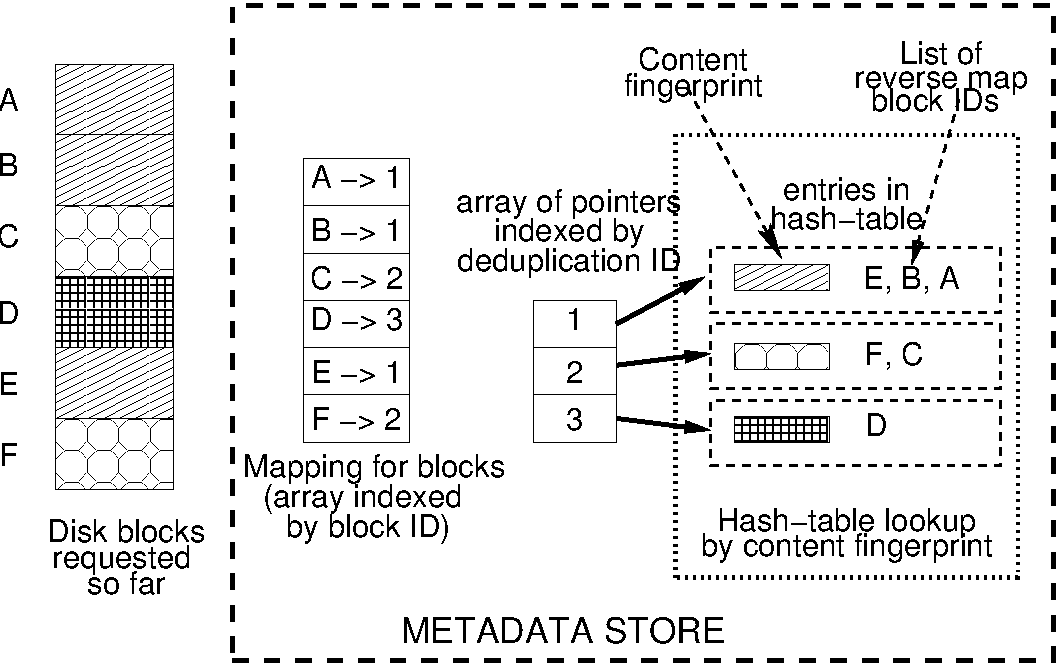
\includegraphics[scale=0.7]{confided-figures/main/metadata-structure.pdf}
    \vspace{-0.1in}
    \caption{Implementation of metadata store: \textit{this figure shows
			the population of various data structures for the example
			introduced earlier in Fig.}~\ref{fig:deduped-block}.}%: \textit{two arrays and a hash-table}}
    \label{fig:metadata-structure}
%    \vspace{-0.2in}
\end{figure}

Duplicate content identification is accomplished using the content fingerprint 
as a key to lookup and find the corresponding hash-table entry.
The fingerprint technique, used for duplicate content identification,
can be MD5\cite{md5}, SHA-1\cite{sha1} or SHA-2\cite{sha2},
or any other technique which can be assumed to be hash collision-resistant.
%has no collisions over the 4096 bytes domain. 
Usage of MD5 or SHA fingerprints to assess content similarity is established
practice in existing work~\cite{similarity, iodedup, idedup, lbfs, venti}
and it is known that probability of (error caused by) a hash-collision in
SHA fingerprinting is much lower than an arbitrary hardware
error~\cite{compare-by-hash}.
It is argued~\cite{compare-by-hash} that ``compare-by-hash''
is not a satisfactory technique to establish block content similarity, with
suggestion to use combination of hash comparison with other methods
like Rabin fingerprinting~\cite{rabin} to ensure correctness.
We use MD5 fingerprints in our prototype implementation, % for simplicity, 
however any collision-resistant fingerprinting module can be plugged
into our implementation and would not have significant impact on the
results presented in this work.


\subsection{Metadata update and implicit hints about host-cache state}
In the case where metadata was not previously available, and a content
buffer has been received from the back-end driver, the DRIVE module
within the front-end driver performs fingerprint comparison into the
hash-table to determine whether the content is unique or a duplicate.
If the content is unique, a new deduplication ID is assigned (say $X$) and a
mapping from block ID $P$ to $X$ is registered, an entry for the new 
deduplication ID
is made into the hash-table with the content's fingerprint as hash key,
and the original block ID $P$ is initialized as the only member of the
list of reverse mappings in that hash-table entry.
On the other hand, if the content is a duplicate, a hash-table 
entry already exists, so the block ID $P$ is added to the associated
list of reverse mappings.

Within the list of reverse mappings associated with each deduplicated
block entry, the most recently fetched duplicate block (\textit{leader}), 
is to be used for I/O redirection. 
To implement this, the list of reverse mappings is maintained in 
Last-in-First-Out (LIFO)\index{LIFO}
\nomenclature{LIFO:}{Last In, First Out}
\nomenclature{FIFO:}{First In, First Out}
order, and block IDs are added to the list
as and when duplicate blocks are encountered.
If the \textit{leader} block content
changes due to a write request, it is removed from the list of reverse
mappings and the next most recently fetched block ID is considered the 
new \textit{leader}.
%\subsubsection{Metadata update upon block writes}
%If the mapping being invalidated was previously the \textit{leader} identified 
%for its corresponding deduplicated block, then after invalidation, the
%next available mapping is marked as the new \textit{leader}.
Continuing with the example of Fig.~\ref{fig:confided-working(a)}, 
if block E (a \textit{leader}) is written, 
metadata for deduplicated block 1 would change,
hence picking a new leader, i.e. the next most recently fetched block B.


\subsection{CPU overhead}
\label{sec:drivechap-cpuoverhead}
Hashing of data, and hash-table lookups
during read and write operations, result in resource overhead.
As compared to Vanilla system, the DRIVE system adds CPU overhead
in following scenarios: (i)~Every read request requires a metadata
lookup for I/O redirection, (ii)~In case of non-existent metadata for a
read request, metadata update is required after data fetch, and 
(iii)~Every write request requires metadata lookup for invalidation. 
We analyze CPU overhead incurred for the two main cases of 
``metadata lookup'' and ``metadata update''.

%In our implementation,
\textit{Metadata lookup} consists of the following three steps.
The \textit{first step} uses block ID as an index into an
array to get the corresponding deduplication ID. If metadata for a block
is non-existent or dirty, the array lookup will fail, however if
metadata exists, the \textit{second step} uses the deduplication
ID to index into another array to get the deduplication entry.
%The deduplication entry corresponds to deduplicated content and is 
%represented by its fingerprint, as discussed earlier.
%Since the deduplication entry contains a list of reverse-mappings also, 
The \textit{third step} is to read the \textit{head} of the list of 
reverse-mappings to get the \textit{leader} block ID for I/O redirection. 
All the above three steps require constant time, hence metadata lookup
times are O(1).

\textit{Metadata update} operation can be of two 
types\textemdash{}creating new metadata for unique blocks, or
modifying existing metadata for duplicate blocks.
The dominating component of the metadata update operation is MD5
hash computation which is known to take around 100,000 CPU
cycles\cite{iodedup} or 33$\mu$s on a 3GHz machine. The computed MD5 hash 
is then used in a hash-table
lookup to locate a hash-table bucket. The hash-table size and
the uniformity of entry distribution across buckets would determine the
number of entries in each bucket. An empty hash-table bucket signifies that
a new entry is to be created. However, if the bucket is non-empty,
%Within the located hash-table bucket,
comparison of MD5 hash to the fingerprint stored within each entry is done
until exact match is found. Higher the number of entries per bucket, longer
this match-lookup time; however given enough number of buckets,
hash-table lookup time would be O(1).


\subsection{Memory overhead}
In our implementation, we use an array indexed by block ID, another
array of pointers indexed by deduplication ID and a hash-table containing
deduplication entries. Assuming a 500GB file system,
the first array
would contain 500GB/4KB = 125,000,000 number of entries of 4 bytes each,
which equals 500MB of space which is too huge.
However, it is observed that only a small
portion of the file system is accessed over long periods of time \cite{iodedup},
hence we can instead use a hash-table implementation to store only those
block IDs which have been requested so far. Thus, using a million-entry
hash-table for block ID lookup, we would need only
4MB of space. However, this change would result in the metadata lookup time
increasing slightly.

Next, we consider the size of the array of pointers indexed by deduplication
ID.
This structure would have only as many entries as there are
deduplicated (or unique) content encountered during read operations.
Assuming that 4 blocks have similar content on average (as reported
in \cite{iodedup}), 4 million blocks read would result in 1 million
deduplication indices. With 8 bytes per pointer, this results in 8MB of space.
Third, we consider the memory used by the hash-table.
Each deduplication entry is associated with an MD5
fingerprint of 16 bytes and a list of reverse-mappings.
Due to content similarity of 4 assumed
above, every deduplication block entry would have a list of size 4, i.e.
16 bytes. Thus, a single deduplication entry would amount to 32 bytes,
and a million such entries would require 32MB.
Thus, the total memory overhead incurred by DRIVE is
%4MB + 8MB + 32MB = 
44MB, which is approximately 4.4\% of 1GB.
\\
\\
Note that a trade-off exists between metadata lookup time and metadata
space usage.
%, in that, lower lookup times can be achieved by using greater
%space for metadata store. 
However, studying this trade-off is not within
current scope, and is left for future work. Nevertheless, we indeed
make a humble attempt to minimize space usage to the extent possible
while achieving constant or O(1) lookup timings.
%An alternative
%implementation which may enable quicker lookups is to directly use a pointer
%from the block mapping to the corresponding entry in the hash-table.
%For example,
%instead of $A \rightarrow 1$ and then pointer indexed by deduplication ID $1$
%pointing to the hash-table entry (say X) in
%Fig.~\ref{fig:metadata-structure},
%there would be a direct pointer $A \rightarrow X$. However, there are two
%drawbacks to this approach. First, this would result in
%each block entry requiring a pointer instead of an index value. Assuming
%a pointer requires 8 bytes compared to an index of 4 bytes\cite{idedup},
%our implementation saves 4 bytes per block entry. Second, this direct
%link would result in a pointer to deduplication block for every block
%entry, whereas our implementation uses a pointer to deduplication block
%only for as many deduplication indices that are present in the system.
%For example, if every block has one duplicate block, this reduces the
%number of such pointers by half.
%For the sake of our prototype implementation, we
%assume infinite space to hold metadata, however, later we evaluate space 
%needed for the same.


